\documentclass[8.01x]{subfiles}
\begin{document}

\chapter{Week 7}

\section{Lecture 15: Momentum and its conservation}

We will now introduce the concept of momentum.\\
Momentum is a vector: the product of mass and velocity. The SI units are then kg $\cdot$ m/s or N $\cdot$ s; there is no named unit for this quantity.

It is usually written as $\vec{p}$, so

\begin{equation}
\vec{p} = m \vec{v}
\end{equation}

Momentum is closely connected with force, and knowing the above, it is easy to show how. $\displaystyle F = m a = m \frac{dv}{dt}$. We can work backwards, assuming $m$ is a constant so that $m \frac{dv}{dt} = \frac{d(mv)}{dt}$:

\begin{equation}
F = m \frac{dv}{dt} = \frac{d(mv)}{dt} = \frac{dp}{dt}
\end{equation}

So force is the time derivative of momentum.\\
This also implies that in order for an object's momentum to change, a force must have acted on it. And, conversely, if a (net) force acts on an object, its momentum must change.

Next, the professor shows (in some detail) how momentum is conserved for a \emph{system} of particles/objects, unless there is a net \emph{external} force on them. What happens internally does not matter, since all such internal forces cancel out, when you consider the system as a whole. For example, if two particles collide, the momentum of both particle \#1 and of particle \#2 may change, but the momentum of \#1 + \#2 will stay a constant.

This then leads to the \emph{conservation of momentum}, which is a very helpful concept in solving some kinds of problems. Let's solve a simple problem using this principle.

Say we have two objects of masses $m_1$ and $m_2$ respectively, both moving towards the right, with velocities $v_1$ and $v_2$, where $v_1 > v_2$. Eventually, the two will collide.

Momentum prior to the collision can be found by the sum $m_1 v_1 + m_2 v_2$; since it is a vector, it has a direction. Both velocities are towards the right, so the net momentum will be as well; we take right to be increasing value of $x$, so that the numbers are positive.

In the collision, the masses will stick together -- pretend that we put glue on one of them. (Collisions where the two separate after colliding are covered later in the lecture, or in the next.)\\
Because they stick together, they will share a velocity later -- and a momentum, as well. The momentum after the collision can be written as $(m_1 + m_2) v'$, if we call the new velocity $v'$. 

Via conservation of momentum, the two must be equal, if there are no external forces (so this collision happens on a frictionless table, with no air drag etc). We set them equal, and solve for $v'$:

\begin{align}
(m_1 + m_2) v' &= m_1 v_1 + m_2 v_2\\
v' &= \frac{m_1 v_1 + m_2 v_2}{m_1 + m_2}
\end{align}

To get a feeling for this, say $m_1 = \SI{1}{kg}$, $m_2 = \SI{2}{kg}$, $v_1 = \SI{5}{m/s}$ and $v_2 = \SI{3}{m/s}$. Mass 1 has a momentum of $\SI{5}{kg m/s}$, while mass 2 has $\SI{6}{kg m/s}$. The net momentum prior to the collision is then $\SI{11}{kg m/s}$, since the two are in the same direction.

Both velocities are towards the right and thus positive, so $v'$ will also be positive.\\
Plugging the numbers in, we find $\SI{11/3}{m/s}$ as the new velocity for the masses, moving together.

What is now the momentum? It is the new velocity times the total mass, which is $(11/3) \times 3$, so indeed we find that momentum was conserved. Not a huge surprise, since we derived the equation from that assumption!

What may be surprising is instead what happens to the kinetic energy.\\
Prior to the collision, the total kinetic energy was 12.5 J + 9 J = 21.5 J.

After the collision, the total kinetic energy is only $20.1\overbar{6}$ J -- we lost one and a quarter of a joule. Not a whole lot, perhaps, but let's look at a second situation.

Say we have the same values for the masses and velocities, only that $v_2$ is now negative, i.e. to the left, and so the two hit each other head-on.

Mass 1 still has the same momentum of $\SI{5}{kg m/s}$, but $v_2$ now has $-\SI{6}{kg m/s}$. The net momentum is now $\SI{-1}{kg m/s}$ instead of +11.

Using the same formula, we now find $v' = -1/3$ m/s. The initial kinetic energy is unchanged -- the masses are the same, and the \emph{speeds} are the same -- but the kinetic energy after the collision is now a tiny 1/6 of a joule!

In short: in the absence of (net) external forces, the momentum of a \emph{system} of two or more objects is always conserved; kinetic energy, however, is not.

Let's have a look at a two-dimensional problem from a lecture question:

``In a scattering experiment, an incident alpha particle of mass $M_1 = 4u$ interacts with a static proton of mass $M_2 = u$. The incident particle is initially moving along the x-axis with a velocity $\vec{v_1} = v_{1x} \hat{x} = 0.05 c \hat{x}$, and a final velocity (after collision) $\vec{v_1}' = v_{1x}^{'} \hat{x} + v_{1y}^{'} \hat{y} = 0.044 c \hat{x} + 0.008 c \hat{y}$, where $c$ is the speed of light ($c = \SI{3e8}{m/s}$).

What is the speed of the proton after the collision?\\
What is the direction of the proton after the collision? (give the angle with respect to the x-axis in radians)''

Haha, honestly, I was stuck for a while, since I found one equation with two unknowns, for each component, so total two equations, four unknowns. It turns out that half of those ``unknowns'' are part of the question, only I didn't realize at first. Duh!

To solve this, we apply conservation of momentum on the two axes, independently of each other.\\
Before and after the collision, in the $x$ direction:

\begin{align}
4 u v_{1x} = 4 u v_{1x}^{'} + u v_{2x}^{'}\\
4 (v_{1x} - v_{1x}^{'}) = v_{2x}^{'}
\end{align}

where $v_{2x}^{'}$ is the $x$ component of the proton's velocity after the collision. Plugging in the numbers given, we find $v_{2x}^{'} = 4(0.05c - 0.044c) = 0.024c$.

Next, the $y$ direction. Neither particle has any $y$ component whatsoever at the moment, so the net momentum prior to the collision is clearly zero. That also means that the net momentum \emph{after} the collision must be zero.

\begin{align}
4 u v_{1y}^{'} + u v_{2y}^{'} = 0\\
v_{2y}^{'} = -4 v_{1y}^{'}
\end{align}

So we find $v_{2y}^{'} = -0.032c$.

With that in mind, we can now calculate the speed as $v_2^{'} = \sqrt{(v_{2x}^{'})^2 + (v_{2y}^{'})^2} = 0.04c$.

Next up, the angle made with the $y$ axis. If we consider the components, it must be angled downwards to the height. Drawing it out, we find that

\begin{equation}
\theta = \arctan \frac{v_{2y}^{'}}{v_{2x}^{'}} = \arctan \frac{-0.032}{0.024} = \ang{-53.13}
\end{equation}

This angle would put it in the correct quadrant, and since the magnitude of the $y$ component is slightly greater than that of the $x$ component, it makes sense that the angle is a bit more than a 45 degrees down from the axis.

Next, there is a great demonstration of the conservation of momentum. I didn't take any notes of it, however.

\subsection{Center of mass}

Every object, regardless of shape or size, has a center of mass; a single point, which has some very interesting and useful properties.

We take any object, of any size (greater that zero, however, or the entire point is lost), and think of it as being composed by a practically infinite amount of small masses $m_i$. Each mass has a position vector $\vec{r_i}$ from the origin, which we are free to choose.

\begin{center}
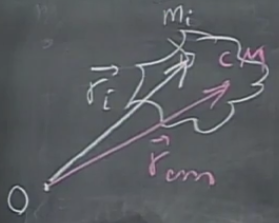
\includegraphics[scale=0.7]{Graphics/lec15_cm}
\end{center}

It is then true that the 

\begin{align}
M_{tot} \vec{r_{cm}} &= \sum_i m_i \vec{r_i}\\
\vec{r_{cm}} &= \frac{1}{M_{tot}} \sum_i m_i \vec{r_i}
\end{align}

In the limit as the masses become infinitesimally small, this becomes an integral:

\begin{align}
\vec{r_{cm}} &= \frac{1}{M_{tot}} \int \vec{r} \mathop{dm}
\end{align}

$x$, $y$ and $z$ components of this can be found in the same way, with three separate integrals.

For the simple case of two particles along a single axis:

\begin{equation}
x_{cm} = \frac{m_1 x_1 + m_2 x_2}{m_1 + m_2}
\end{equation}

This gives a result where the center of mass is closer to the more massive of the two objects. If they are equally massive, the center of mass is at the midpoint between the two.

Returning to the first equation solved for $\vec{r_{cm}}$, we can take the time derivative of both sides of this equation. $\vec{r_{cm}}$ becomes $\vec{v_{cm}}$, and $\vec{r_i}$ becomes $\vec{v_i}$, since velocity is the time derivative of position.

\begin{equation}
\vec{v_{cm}} = \frac{1}{M_{tot}} \sum_i m_i \vec{v_i}
\end{equation}

However, note that $\sum_i m_i \vec{v_i}$ is the sum of the mass-velocity products: it is the total momentum of the system. In other words,

\begin{align}
\vec{v_{cm}} &= \frac{1}{M_{tot}} \vec{p_{tot}}\\
\vec{p_{tot}} &= M_{tot} \vec{v_{cm}}
\end{align}

This second result is an important one: the total momentum of a system can be found by knowing its total mass and the velocity of its center of mass, and is the same regardless of what the rest of the system is doing.

Not only that, but we can take the time derivative of this. The time derivative of momentum is force (or net external force, to be more precise), while the derivative of velocity of the center of mass is the \emph{acceleration} of the center of mass:

\begin{equation}
F_{ext} = M_{tot} \vec{a_{cm}}
\end{equation}

This is a very interesting result. Regardless of the shape of an object, if we know the external force and the total mass, we can predict how the center of mass moves in a simple way, even though the motion of the object as a whole may be very complicated and involve tumbling/spinning at varying speeds, etc.

So if the (net) external force is zero, the center of mass will continue to move in a straight line, forever, regardless of what the rest of the object is doing.

\section{Lecture 16: Elastic and inelastic collisions}

Last lecture was focused on inelastic collisions; we will now consider general collisions, including elastic ones. Again, let's start with a one-dimensional example.

A mass $m_1$ is moving towards the right with speed $v_1$, towards a mass $m_2$ which is at rest. We take increasing values of $x$ to be towards the right.

After the collision, $v_1^{'}$ can be either positive or negative (to the right or to the left), while $v_2^{'}$ is certainly towards the right. (If an object hits it from the left, how could it start moving towards the left?)

To find the velocities after the collision, we can apply conservation of momentum. Only the first mass had any momentum prior, so that must be the sum of the momentum after the collision as well:

\begin{equation}
m_1 v_1 = m_1 v_1^{'} + m_2 v_2^{'}
\end{equation}

Unfortunately, the equation has two unknowns; we need a second equation to get anywhere.

In order to find a second equation, we can use the conservation of energy. \emph{Kinetic} energy is not necessarily conserved in collisions, which we saw last lecture. However, the kinetic energy that is lost must be converted to some other form of energy, such as heat energy.

If we use an extra $Q$ to denote the rest of the energy, we can write an equation of the form $K + Q = K'$, where $K$ is the kinetic energy prior to the collision, and $K'$ is the kinetic energy after.

There are three possible cases here.

\begin{itemize}
\item $Q > 0$: we call this a \emph{superelastic} collision; the amount of kinetic energy has \emph{increased} (as demonstrated with a spring's stored energy as the source in the previous lecture; an explosion or such could also cause this to happen).
\item $Q = 0$: this is an \emph{elastic} collision (or ``completely elastic''; the modifier ``completely'' is really not necessary, however). Kinetic energy is \emph{conserved} in this special case.
\item $Q < 0$: this is an inelastic collision. Kinetic energy is lost in the collision (in any amount from almost none lost, to \emph{all} kinetic energy lost), and is mostly turned into heat (but perhaps also noise and vibration, etc).
\end{itemize}

Let's focus on the special case of elastic collision, so that $Q = 0$ and $K = K'$. In this case, we can write an equation relating the initial kinetic energy to the final kinetic energy, as follows:

\begin{align}
\frac{1}{2} m_1 v_1^2 &= \frac{1}{2} m_1 (v_1^{'})^2 + \frac{1}{2} m_2 (v_2^{'})^2\\
m_1 v_1^2 &= m_1 (v_1^{'})^2 + m_2 (v_2^{'})^2
\end{align}

Combining this with the equation that relates the momentum of the system, we can find expressions for $v_1^{'}$ and $v_2^{'}$ as follows, by solving the system of equations:

\begin{align}
v_1^{'} &= \left(\frac{m_1 - m_2}{m_1 + m_2}\right) v_1\\
v_2^{'} &= \left(\frac{2 m_1}{m_1 + m_2}\right) v_1
\end{align}

So the above is valid under three conditions: the initial velocity $v_2 = 0$ initially, $Q = 0$ and momentum is conserved (i.e. there is no net external force on the system).

We will now look at what will happen in three special cases: $m_1 \gg m_2$, $m_1 \ll m_2$ and $m_1 = m_2$.

First out is $m_1 \gg m_2$, which turns out to be the same as $m_2 \to 0$. What happens in the above equations as $m_2 \to 0$?

Well, $v_1^{'} = v_1$ -- which comes as no surprise. If a very massive object runs in to one that has practically zero mass, it will just continue on its way.\\
What happens to the smaller object is more interesting: its velocity goes to $v_2^{'} = 2 v_1$. As long as $m_1 \gg m_2$, no matter what the actual masses or velocities are, it will zoom away at twice the speed of the object that hits it.

Next, the opposite case, where $m_1 \ll m_2$, which means $m_1 \to 0$. Since $m_1$ is the one that moves initially, I would expect it to change direction and move backwards at some speed, while $m_2$ does almost nothing. Let's plug it in: we find $v_1^{'} = -v_1$ and $v_2^{'} = 0$, as predicted. It turns out that $m_1$ simply bounces back with the \emph{same} speed, only in the opposite direction. Considering what happened to the tiny mass in the previous case, this might not be obvious -- it was twice the speed in the previous case!

Finally, what happens if the masses are about the same? Plugging it in, we find $v_1^{'} = 0$, and $v_2^{'} = v_1$: the first object stops, and the second moves as the first one did prior to the collision.\\
Most have seen this in action, perhaps while playing pool, or in a ``Newton's cradle'' where several balls (usually at least 3, but 2 works) hang suspended as pendula; you raise one up, and when it whacks on the rest, only the one at the other end starts moving; the others merely ``relay'' the momentum through until it reaches the last ball.

The cases where $m_1 = m_2$ and $m_1 = 0.5 m_2$ are then demonstrated, with very convincing results!

What if $v_2 \neq 0$? More specifically, $v_2 > 0$, so that they are both moving towards the right, with $v_1 > v_2$ so that they will eventually collide. Again, we assume an elastic collision.

If we set up the system of equations, with the change that both masses now have momentum towards the right, and both have initial kinetic energy, we find 

\begin{align}
v_1^{'} &= \frac{m_1 v_1 - m_2 v1 + 2 m_2 v_2}{m_1 + m_2}\\
v_2^{'} &= \frac{2 m_1 v_1 - m_1 v_2 + m_2 v_2}{m_1 + m_2}
\end{align}

With $m_1 = m_2$, this yields a funny result: the two essentially trade speeds with one another. $v_1^{'} = v_2$ and $v_2^{'} = v_1$.

\subsection{Elastic collisions seen from the frame of the center of mass}

We can choose our reference frame such that the center of mass has zero velocity in our frame. This is referred to as the ``center of mass frame'', ``center of momentum frame'' or COM frame.

In this frame, total momentum is always zero. We found last lecture that $\vec{p_{tot}} = M_{tot} \vec{v_{cm}}$, and \emph{in the COM frame}, $v_{cm} = 0$ by definition. That definition is what makes it the COM frame.

Using the definition for the velocity of the center of mass

\begin{equation}
v_{cm} = \frac{1}{M_{tot}} \sum_i m_i v_i = \frac{\sum_i m_i v_i}{\sum_i m_i}
\end{equation}

and a Galilean transformation for the velocities of two particles,

\begin{align}
u_1 &= v_1 - v_{cm}\\
u_2 &= v_2 - v_{cm}
\end{align}

where the $u$ notation is used for the particle's velocities in the COM frame, we can show that the total momentum must be zero in this frame, in a different way.

The sum $\sum_i m_i u_i$ is the net momentum in the COM frame. $u_i = (v_i - v_{cm})$, so we substitute that in and find $\sum_i m_i (v_i - v_{cm})$ as the total momentum. Using the definition of $v_{cm}$ above, that is

\begin{equation}
\sum_i m_i \left(v_i - \frac{\sum_i m_i v_i}{\sum_i m_i}\right) = \sum_i m_i v_i - \sum_j m_j \frac{\sum_j m_j v_j}{\sum_j m_j} = 0
\end{equation}

The denominator in the fraction becomes $1$, and we then have the subtraction of two equal quantities that equals the total momentum, as seen from the COM frame, since the indices $i$ and $j$ are equivalent.

Now that we can hopefully accept the above as being true (I had trouble seeing it until I did the above)...\\
Say we are in this frame, and there are two particles with velocities inward toward the center of mass; one mass $m_1$ with speed $u_1$, and one mass $m_2$ with speed $u_2$ -- again with those speeds being in the COM frame. Also say $Q = 0$ for this collision, i.e. it is an elastic collision.

Momentum is zero both before and after the collision. In addition, because this is an elastic collision, we can also write down an equation relating kinetic energy before and after the collision. Altogether, we have:

\begin{align}
m_1 u_1 + m_2 u_2 &= 0\\
m_1 u_1^{'} + m_2 u_2^{'} &= 0
\end{align}
\begin{equation}
\frac{1}{2} m_1 u_1^2 + \frac{1}{2} m_2 u_2^2 = \frac{1}{2} m_1 (u_1^{'})^2 + \frac{1}{2} m_2 (u_2^{'})^2
\end{equation}

With all this information, we can find (through some tedious algebra) two very simple answers: $u_1^{'} = -u_1$ and $u_2^{'} = -u_2$.

That is, \emph{as seen from the center of mass frame}, which is moving, both simply reverse direction, but keep moving at the same speed. This happens regardless of the masses and speeds, so this is clearly only possible in this very special frame.

In this simple case with only two objects, the definition we have above for $v_{cm}$ is fairly simple:

\begin{equation}
v_{cm} = \frac{m_1 v_1 + m_2 v_2}{m_1 + m_2}
\end{equation}

We can then follow the process of first transforming our velocities into velocities as seen from the center-of-mass by subtracting $v_{cm}$, do the collision calculations knowing that momentum is zero both before and after the collision (this holds for all collisions; inelastic, elastic and superelastic), and then transforming back to the external frame by \emph{adding} $v_{cm}$ back.

Since the center of mass moves at a constant velocity in the absence of external forces, we need not worry about it having changed during the collision (unless we are making an incorrect assumption that the external forces are zero).

Let's try an example (from a lecture question).

``Before a 1-dimensional collision, two masses $m_1 = 3$ kg and $m_2 = 5$ kg have velocities $v_1 = -5$ m/s and $v_2 = 3$ m/s with respect to their center-of-mass frame.

What are their velocities (in m/s) in the laboratory frame after an elastic collision? (The velocity of the center of mass is $v_{cm} = 2$ m/s)''

Alright, so in the center of mass frame, $v_1^{'} = 5$ m/s and $v_2^{'} = -3$ m/s, since all they do in that frame is reverse direction. To convert this to the lab frame, we need to \emph{add} $v_{cm}$ to these numbers, so we find 7 m/s and -1 m/s, respectively. That was certainly very easy.

\subsection{Inelastic collisions seen from the center of mass frame}

The center of mass frame has another interesting property. In the case of a completely inelastic collision, i.e. the two masses that collide stick together, both velocities go to zero (as seen from the center of mass; this would be true even if they were sliding together according to an outside observer).\\
Zero velocity means zero kinetic energy, so \emph{all} kinetic energy will be lost in this frame.

This kinetic energy, as seen from the center of mass frame, is called the \emph{internal energy}; it is the maximum energy that can be converted to heat in a collision.

Let's first calculate the amount of kinetic energy lost in a completely inelastic collision, as seen from the ``lab frame'' (one that is fixed to the room you're in, i.e. what at least I personally would consider the default frame).

We take the case where a mass $m_1$ moves with speed $v_2$ towards a second mass, $m_2$, that is at rest (with respect to the lab frame). It's a completely inelastic collision, so they stick together after the collision.

After the collision, we call the velocity $v'$ (which is just a speed in the same direction as $v_1$, since momentum is conserved), and the total mass is then $m_1 + m_2$.\\
Conservation of momentum gives

\begin{equation}
m_1 v_1 = (m_1 + m_2) v'
\end{equation}

\begin{equation}
v' = \frac{m_1 v_1}{m_1 + m_2}
\end{equation}

$v_{cm} = v'$; that can be seen very easily by looking at the equation for $v_{cm}$, and considering the case where $v_2 = 0$, as it is here. $v_{cm}$ equals exactly the above expression in that case.

Next, we can calculate the difference is potential energy before ($K$) and after ($K'$) the collision. This is the $Q$ we had in a previous equation (see the note just below; I made a small mistake):

\begin{align}
Q = K' - K &= \frac{1}{2} m_1 v_1^2 - \frac{1}{2} (m_1 + m_2) \left(\frac{m_1 v_1}{m_1 + m_2}\right)^2\\
           &= \frac{1}{2} m_1 v_1^2 - \frac{m_1^2 v_1^2}{2(m_1 + m_2)}\\
           &= \frac{m_1 v_1^2(m_1 + m_2)}{2(m_1 + m_2)} - \frac{m_1^2 v_1^2}{2(m_1 + m_2)}\\
           &= \frac{m_1 v_1^2(m_1 + m_2) - m_1^2 v_1^2}{2(m_1 + m_2)}\\
           &= - \frac{m_1 m_2}{2(m_1 + m_2)} v_1^2 \text{ (see below re: minus)}
\end{align}

Phew! This is then, from the external reference frame, the amount of kinetic energy lost in the collision.\\
As it turns out, I accidentally calculated $K - K'$ instead. The only difference is a minus sign, of course, so the actual answer should be \emph{minus} what I actually found; I added the sign in the last step above, instead of re-writing the code for this mess; sorry about that.\\
So the last line in the equation above is correct.

Next, we do the same calculation in the center of mass frame. We know $v_{cm}$, $v_1$ and $v_2$, so we can jump straight to converting the velocities. Using $u_i$ for the velocities as seen from the center of mass frame,

\begin{align}
u_1 &= v_1 - v_{cm} = v_1 - \left(\frac{m_1 v_1}{m_1 + m_2}\right)\\
u_2 &= v_2 - v_{cm} = - \left(\frac{m_1 v_1}{m_1 + m_2}\right)
\end{align}

The first equation simplifies:

\begin{align}
u_1 &= \frac{v_1(m_1 + m_2) - m_1 v_1}{m_1 + m_2}\\
u_1 &= \frac{v_1 m_1 + v_1 m_2 - m_1 v_1}{m_1 + m_2}\\
u_1 &= \frac{v_1 m_2}{m_1 + m_2}
\end{align}

And we can then write them as

\begin{align}
u_1 &= \left(\frac{m_2}{m_1 + m_2}\right) v_1\\
u_2 &= - \left(\frac{m_1}{m_1 + m_2}\right) v_1
\end{align}

We can then calculate the total kinetic energy \emph{prior} to the collision as

\begin{align}
K &= \frac{1}{2} m_1 u_1^2 + \frac{1}{2} m_2 u_2^2\\
K &= \frac{1}{2} m_1 \left(\left(\frac{m_2}{m_1 + m_2}\right) v_1\right)^2 + \frac{1}{2} m_2 \left(- \left(\frac{m_1}{m_1 + m_2}\right) v_1\right)^2\\
K &= \frac{1}{2} m_1 \left(\frac{v_1 m_2}{m_1 + m_2}\right)^2 + \frac{1}{2} m_2 \left(\frac{v_1 m_1}{m_1 + m_2}\right)^2\\
K &= \frac{v_1^2 m_1 m_2^2}{2(m_1 + m_2)^2} + \frac{v_1^2 m_2 m_1^2}{2(m_1 + m_2)^2}\\
K &= \frac{v_1^2 m_1 m_2^2 + v_1^2 m_2 m_1^2}{2(m_1 + m_2)^2}\\
K &= \frac{(m_1 + m_2) m_1 m_2 v_1^2}{2(m_1 + m_2)^2}\\
K &= \left(\frac{m_1 m_2}{2(m_1 + m_2)}\right) v_1^2
\end{align}

Again, phew! Note that this is exactly the same as the answer we found earlier, for the kinetic energy lost in the lab frame.\\
In this frame, that energy is \emph{all kinetic energy that exists to begin with}. After the collision, kinetic energy will be zero, since the wreck sticks together (this entire section is about a completely inelastic collision), and neither body will move with respect to the center of mass after the collision.\\
In other words, the \emph{change} in kinetic energy is the same in both reference frames, even though the initial and final energies are different in the different frames.

Lecture question time.

``Just before an inelastic head-on collision, two cars have a relative speed of $v = 40$ km/h (25 mph). The cars have masses $m_1 = 1300$ kg and $m_2 = 1600$ kg.\\
How much kinetic energy is lost during the collision?''

Hmm. Well, we can use the equation above. Assume $v_2 = 0$, and then it's just a matter of sticking the numbers in there, which yields about 44300 J.

\section{Lecture 17: Momentum of individual objects}

Previously, we measured the speed of a bullet, simply by measuring how long it took the bullet to move a certain distance. This was only possible because of the electronic timer, which both started and stopped automatically, as the bullet was shot through two wires.\\
We will now calculate the speed, by a more manual, indirect method, of firing the bullet into a block hanging as a pendulum. This way, we can find the velocity (with a fairly large uncertainty, but still) with nothing but a small meter stick and knowledge of physics.

The way in which we do this is fairly complex, but let's start simple. We have a solid block of mass $M$ hanging from a string of length $\ell$; this forms a \emph{ballistic pendulum}.

The bullet of mass $m$ comes in with a velocity $v$, and ``merges'' with the block (gets stuck inside), so we can model this is a completely inelastic collision. The block moves from its equilibrium position (straight down), towards the right and slightly upwards (since it is a pendulum!), with velocity $v'$.

We can apply conservation of momentum to find $v'$:

\begin{align}
m v &= (m + M) v'\\
v' &= \frac	{m v}{m + M}
\end{align}

Soon thereafter, $v'$ will have gone to zero, as the pendulum reaches its highest point. Here, we know that kinetic energy is zero, and all kinetic energy has been converted into gravitational potential energy.\\
If we define $U = 0$ at the equilibrium position, the change in gravitational potential energy was $(m + M) g h$, where $h$ is the amount the block moved upwards. This energy must have come from the kinetic energy, so via conservation of energy, we can relate the block's initial kinetic energy (as the bullet is absorbed) and the gravitational potential energy as it stops:

\begin{equation}
\frac{1}{2} (m + M) (v')^2 = (m + M) g h
\end{equation}
\begin{equation}
v' = \sqrt{2 g h}
\end{equation}

With this in mind, we could theoretically fire a bullet into the block, measure how far it moves up, and calculate the speed of the bullet. However, the upwards movement is minuscule, less than a single millimeter; we still cannot measure that with any useful accuracy. We \emph{can} measure how far it travels towards to the side, though, since that excursion is must greater. (Remember how we even neglected the upwards motion of a pendulum completely when we derived an equation for it using simple harmonic motion?)

So if we set the origin at the equilibrium position, we can call the maximum horizontal displacement of the pendulum $x$. Via trigonometry, we can find that $x = \ell \sin \theta$, and $h = \ell - \ell \cos \theta = \ell(1 - \cos \theta)$.

Using the same small-angle approximations we have used previously, that $\displaystyle \cos \theta \approx 1 - \frac{\theta^2}{2}$ and $\sin \theta \approx \theta$ (both only valid for radians), $\displaystyle h \approx \ell \frac{\theta^2}{2}$.

For $\ell = 1$ meter and $\theta = \ang{2}$, we find that $h \approx 0.6$ mm, far to small to measure with any useful accuracy. However, $x \approx \ell \theta \approx 3.5$ cm, which is much more reasonable. 

Since we now know $x$ as a function of $\theta$, we can write $h$ as a function of $x$ by combining the two equations:

\begin{equation}
h \approx \ell \frac{\theta^2}{2} \approx \frac{\ell}{2} \left(\frac{x}{\ell}\right)^2 = \frac{x^2}{2 \ell}
\end{equation}

With this in mind, we can find $v'$ as a function of $x$

\begin{equation}
v' = \sqrt{2 g} (\frac{x}{\sqrt{2 \ell}}) = x \sqrt{\frac{g}{\ell}}
\end{equation}

... and then finally the bullet's original velocity $v$ as a function of $v'$, by using the old conservation of momentum equation we had:

\begin{equation}
v = \frac{v'(m + M)}{m} = x \frac{m + M}{m} \sqrt{\frac{g}{\ell}}
\end{equation}

Let's now look at some numbers. The mass of the bullet is $m = \SI{2.0(2)}{g}$; $M = \SI{3.20(2)}{kg}$, and $\ell = \SI{1.13(2)}{m}$.

With these numbers, we find $v = 4.7 \times 10^{3} x$. The total uncertainty is somewhere around 15\%, in large part because of the large uncertainty in $m$.

When the experiment is carried out, $x \approx \SI{5.2}{cm}$ = 0.052 meters, so $v \approx \SI{244}{m/s}$. Of course, with a 15\% uncertainty, that last four may be rather meaningless. 15\% less than this is just 207.5 m/s, and 15\% more is 280.5 m/s.

Comparing the initial kinetic energy of the bullet $\displaystyle \frac{1}{2} m v^2 \approx 59.5$ J (with a large uncertainty) and the maximum kinetic energy of the block-bullet system $\displaystyle \frac{1}{2} (m + M) (v')^2 \approx 0.038$ J, we see that the vast majority of the kinetic energy was lost to heat, deforming the block (and perhaps bullet), etc. About 99.94\% was lost, according to the lecture, which seems to match this calculation quite well.

\subsection{Impulse}

Impulse is a concept closely related to momentum. Any time a change in momentum occurs for an object, an impulse was imparted on that object.\\
It is a vector, and can be written as the time integral of force:

\begin{equation}
\vec{I} = \int_{t_0}^{t_1} \vec{F} \mathop{dt} = \int_0^{\Delta t} \vec{F} \mathop{dt}
\end{equation}

using $\Delta t = t_1 - t_0$. In the simple case where the force is constant, $\vec{I} = \vec{F} \Delta t$.

However, force is also the rate of change of momentum. Therefore, the integral above can also be written as the integral of the derivative of momentum -- clearly, the dimension here is going to be the same as that of momentum.\\
In fact, we can show that the impulse is just the difference in momentum at two different times; using $\vec{p_i}$ for the initial momentum and $\vec{p_f}$ for the final momentum, 

\begin{equation}
\vec{I} = \vec{p_f} - \vec{p_i}
\end{equation}

The units of impulse are then the same as those of momentum: kg m/s or newton-seconds ($N \cdot s$).

As an example, take the collision of a ball bouncing on the floor. In the simple case where the collision is elastic, and the ball bounces back to the same height (which is of course impossible, but we can come close), the ball hits the floor with momentum $m v$, if we take downwards to be the positive direction, and leaves with equal momentum in the opposite direction, that is, $- m v$.

The impulse is then found as $- mv - (mv) = - 2 m v$. The impulse is upwards in this case, and has the magnitude of the change in momentum $2 m v$.

In the case of a completely inelastic collision (in other words, no bounce), as with a tomato hitting the floor, the impulse is smaller in magnitude at just $m v$ -- the colliding object loses all of its momentum to the floor, and ends up with zero speed and zero momentum.

Using the definition of impulse in terms of force, we can calculate the average force on a body during a collision as

\begin{equation}
\Braket{F} = \frac{I}{\Delta t}
\end{equation}

As an example, a ball (bouncy ball, super ball or what you may call it) with a mass $m = 0.1$ kg is dropped from a height of 1.5 meters. That gives it a speed of about 5.5 m/s (a bit less) as it hits the floor. Assuming an elastic collision, $I = 2 m v = 1.1$ kg m/s.\\
We can then divide this by the impact time to find the average force. The impact time was measured (by high-speed photography) to be just 2 milliseconds. That gives an average force of

\begin{equation}
\Braket{F} = \frac{\SI{1.1}{kg m/s}}{\SI{0.002}{s}} = \SI{550}{N}
\end{equation}

Remember that our definition (at least one definition) of \emph{weight} was the magnitude of the normal force exerted by e.g. the floor, to counteract gravity. (It could also be the tension in a rope, pulling you upwards.)

That means that this ball, during the short moment of the collision, has a weight about 550 \emph{times} greater than it would otherwise ($550 g$), since its ``normal'' weight is just $m g \approx 1$ N (a bit less, but we use $g \approx \SI{10}{m/s^2}$ for simplicity).

Lecture question time:\\
Car 1 of mass $m_1$ is moving along the +$x$-axis with speed $v_1$ towards car 2 of mass $m_2$ and speed $v_2$ moving along the -$x$-axis. They have a head-on collision that lasts a time interval $\Delta t$. After the collision the cars stick together. (Note: $m_1$ and $m_2$ include the drivers.)

The magnitude of the average force acting upon the driver of mass $m_{dr1}$ in car 1 by her seat belt during the collision is given by:

\begin{align}
F_{dr1} &= \frac{m_1}{m_1 + m_2} (v_1 - v_2) \frac{m_{dr1}}{\Delta t}\\
F_{dr1} &= \frac{m_1}{m_1 + m_2} (v_1 + v_2) \frac{m_{dr1}}{\Delta t}\\
F_{dr1} &= \frac{m_2}{m_1 + m_2} (v_1 - v_2) \frac{m_{dr1}}{\Delta t}\\
F_{dr1} &= \frac{m_2}{m_1 + m_2} (v_1 + v_2) \frac{m_{dr1}}{\Delta t}
\end{align}

If $v_1 = v_2$, considering the two are \emph{speeds} in opposite directions, the driver will most certainty not experience zero force, so the two options with minus signs should both be wrong. Still, let's solve this the proper way.

Total momentum is conserved, and the cars stick together. Considering that $v_2$ is towards the $-x$ axis, its velocity is negative, so the sum of momenta becomes a subtraction. The velocity after the collision is given by

\begin{align}
m_1 v_1 - m_2 v_2 = (m_1 + m_2) v'\\
v' = \frac{m_1 v_1 - m_2 v_2}{m_1 + m_2}
\end{align}

The driver's initial and final speeds are the same as the car's, of course. With that in mind, we can calculate the impulse of the driver directly, as

\begin{align}
I &= m_{dr1} v' - m_{dr1} v_1\\
I &= m_{dr1}  \frac{m_1 v_1 - m_2 v_2}{m_1 + m_2} - m_{dr1} v_1\\
I &= - \frac{m_2(v_1 + v_2)}{m_1 + m_2} m_{dr1}
\end{align}

We wanted a magnitude, but got a negative number; that is simply due to the coordinate system choice. Since all variables must be positive ($v_1$ and $v_2$ are speeds and never negative), we can simply remove the minus sign to find the magnitude.

By definition, $\Braket{F} \Delta t = I$, so we can write this in terms of an average force. We just make that substitution, and solve for the force by dividing both sides by $\Delta t$:

\begin{equation}
\Braket{F} = \frac{m_2(v_1 + v_2)}{m_1 + m_2} \frac{m_{dr1}}{\Delta t}
\end{equation}

Finally, we have one of the four possible answers, and it is indeed the correct one.

Next up, we have some talk about impact times, though nothing general enough to really write down. As always, no notes doesn't mean not worth watching -- it's really a bit of the opposite.

\subsection{Thrust and rockets}

Consider the case of throwing tomatoes towards the floor again. Say we throw $n$ tomatoes per second, and each tomato has a mass $m$. $n m$ is (tomatoes/second) times (kilograms/tomato), so the dimension of this is in kilograms per second of ``stuff'' we throw.

The change in momentum for each tomato is $m v$; $n m v$ gives us the dimension of impulse per time, so

\begin{equation}
n m v = \frac{\Delta p}{\Delta t} = \Braket{F}
\end{equation}

Since $\displaystyle \frac{dp}{dt}$ is the definition of force, the above yields a time-averaged force. The floor experiences a net downwards force from all these tomatoes.

In the form of a proper derivative, we have

\begin{equation}
F = \frac{dm}{dt} v
\end{equation}

Similarly, in the case of a more horizontal case, we need to accelerate these tomatoes from a velocity of 0 to a horizontal velocity of $v_x$. The object they hit (a poor person's face, in the lecture) experiences a force in the same direction as the tomatoes' velocity vector, which should be quite intuitive. Why does this happen, though?\\
Well, the tomatoes come in with velocity $v_x$ and momentum $m v_x$. They hit the person, and all of a sudden $v_x = 0$, and they have lost all of their momentum. Momentum is conserved (there is no relevant external force involved in the horizontal direction), so the momentum is imparted on the person. Since a change in momentum is a force by definition, the person experiences a force in the same direction as their gain in momentum -- away from the tomato thrower.

However, for reasons of symmetry, when we \emph{throw} the tomatoes, they start with zero velocity. It is up to us to give them that velocity $v_x$, and with that, the momentum $m v_x$. Momentum is conserved for us, too, so \emph{we} must experience a change in momentum opposite to that of the tomatoes, so that the sum is zero. Again, a change in momentum is a force -- we feel a force backwards!\\
This too should be fairly intuitive. Recoil from firing a gun is one example of this in effect.

This is, then, how a rocket works. It ejects massive amount of gas, at an extremely high velocity. Both $\displaystyle \frac{dm}{dt}$ and $v$ are high, and the force generated is enormous. This then yields a forward (or upward) \emph{thrust}, which is essentially the reaction force caused by ejecting all that matter.

Note that the thrust of the rocket is not dependent on the ejected matter hitting anything; it works just the same in the vacuum of space.\\
Helicopters work on the practically same principle, only that the air they eject is not stored as a fuel, but simply sucked in from above. Helicopters \emph{do} have a stronger lift near the ground, due to an unrelated effect called the ground effect. With that said, helicopters don't depend on this effect to fly -- if they did, they could only fly at very low altitudes. In fact, the effect is almost completely negligible at a height where the rotor's distance to the ground is greater than the rotor diameter, so the effect becomes irrelevant at about 20 meters off the ground.

As on example, the Saturn V rocket, the exhaust velocity was on the order of 2.5 km/s (!), and about 15000 kg/s of material was spewed out. The net thrust is then the product of the two, about 37.5 million newtons. That sounds like an incredible lot, of course, but the thrust-to-weight ratio (which clearly must be greater than 1 to take off vertically, or gravity would win) was only about 1.2:1 at liftoff. That is still enough to have a net acceleration, though, so that it could reach a speed of 2.7 km/s in less than 3 minutes (and the speed only increased from there, to a bit over 7 km/s).

So this thrust then imparts a impulse on the rocket. The force (the thrust) acts for a certain time, the burn time. However, as the rocket accelerates, the mass of the rocket goes down, since the fuel is being burned and ejected. That in turn causes the acceleration to increase, and so it gains velocity faster. (If the force is constant, and the mass goes down, acceleration must go up. The force is not constant though, but increases; more on that later, I believe.)

\subsection{Velocity change in a rocket}

Let's look at calculating the change in velocity for a rocket, using an approach based on the conservation of momentum.

Consider the rocket at a time $t$. It is moving upwards with a velocity $v$ (relative to an observer on the ground), and has a mass $m$.\\
A short time $\Delta t$ later, the velocity is now $v + \Delta v$, and the mass $m - \Delta m$, since some of the fuel has been burned and ejected to create thrust.

If we use $u$ to denote the exhaust velocity \emph{relative to the rocket} (all other velocities are relative to the ground), the piece of exhaust is moving upwards with velocity $v - u$ as seen from the ground.

If the rocket's velocity is larger than the exhaust velocity, we see the exhaust moving upwards; if not, we see it moving downwards. Both are possible cases, and both are handled by the signs, with positive being upwards.

In the case where no external forces has acted on the system (we will look at gravity soon), momentum is conserved. The rocket's momentum will change for sure, but there will be an equal and opposite change in the exhaust's momentum, such that the net momentum is conserved.

At time $t$, the momentum is $m v$. At the later time $t + \Delta t$, the momentum is still mass times velocity, which is $P_{after} = (m - \Delta m)(v + \Delta v) + \Delta m(v - u)$. The last term is the momentum of the exhaust, which we must not forget!\\
Multiplied out, this is $P_{after} = m v + m \Delta v - v \Delta m - \Delta m \Delta v + v \Delta m - u \Delta m$. 

$v \Delta m$ cancels out, and $\Delta m \Delta v$ is the product of two tiny numbers, so we neglect it. We find the momentum as

$P_{after} = m v + m \Delta v - u \Delta m$.\\
The net change in momentum must be zero, since momentum is conserved. $\Delta p = p_f - p_i$, so $\Delta p = m \Delta v - u \Delta m = 0$.

Considering the case where $\Delta t \to 0$, we can take the time derivative of the above equation, and find

\begin{align}
0 &= m \frac{dv}{dt} - u \frac{dm}{dt}\\
0 &= m a - u \frac{dm}{dt}
\end{align}

Since we previously had the definition that $\displaystyle F_{thrust} = u \frac{dm}{dt}$, where $u$ is the exhaust velocity relative to the rocket, what we really found is

\begin{equation}
F_{thrust} = m a
\end{equation}

What happens if we consider gravity? In a still simplified case, we consider a fully vertical launch. The thrust and the force due to gravity $m g$ are then in exactly opposite directions.\\
We would then find that $m a = F_{thrust} - m g$.

In a derivation not shown, we can then find the change in velocity $\Delta v = v_f - v_i$ (this $\Delta v$ is the \emph{total} change in velocity during the entire burn time of minutes (or so), and has nothing to do with the tiny $\Delta v$'s in the derivation above, over a tiny time period $\Delta t$).

\begin{equation}
\Delta v = -u \ln \frac{m_f}{m_i} - m g
\end{equation}

This then only holds in a fully vertical launch. Since $m_i > m_f$ (the fuel used up will cause the final mass $m_f$ to be much smaller than the initial mass $m_i$), this equation will always be positive, assuming the thrust is greater in magnitude than the force of gravity. If it is not, then clearly, the rocket will either slow down in its upwards motion, or speed up in its fall back to Earth. We could rewrite the signs with this in mind, and flip the fraction inside the natural logarithm:

\begin{equation}
\Delta v = u \ln \frac{m_i}{m_f} - m g
\end{equation}

If we remove the $- m g$ term, this equation is known as the rocket equation (or ideal rocket equation, or Tsiokovsky rocket equation).

According to this equation, the change in the velocity is fixed for a certain amount of fuel burned (assuming $u$ is constant). However, the change in kinetic energy is \emph{not} fixed. In other words, burning the same amount of fuel, in the same rocket, for a certain amount of time will cause a fixed increase in velocity, but the increase in kinetic energy will be \emph{different} for different such burns, depending on the initial velocity!

Consider the increase in kinetic energy from a velocity of 0 m/s to 100 m/s; the increase is $\frac{1}{2} m 100^2$ J. If the rocket instead already has a velocity of 1000 m/s, and we perform exactly the same burn -- same amount of fuel, same exhaust velocity, same burn time and same increase in velocity of 100 m/s (so that the new velocity is 1100 m/s) -- the increase in kinetic energy is now $\Delta K_e = \frac{1}{2} m 1100^2 - \frac{1}{2} m 1000^2 = \frac{1}{2} m (2.1 \times 10^5)$! The increase in kinetic energy is \emph{21 times greater}, and the only difference was the initial velocity. Very non-intuitive!

There is one fairly intuitive way to think about this, though. Work is force times distance; consider the thrust as the force. As the rocket starts out, it is standing still, so the thrust does zero work to begin with. The faster the rocket moves, the greater the distance moved per unit time is (obviously, since that's the definition of speed), and so the amount of useful work is greater at higher speeds.

\end{document}